\sectionquestion{CNNs \& RNNs}

\begin{parts}

\part For this question, you will consider the following kernel: 

\begin{center}
    \begin{tabular}{ |c|c|c| } 
     \hline
     -1 & -1 & -1 \\ \hline
     -1 & 1 & 1 \\ \hline
     -1 & 1 & 1 \\ \hline
    \end{tabular}
\end{center}

\begin{subparts}
    \subpart[1] \textbf{Numerical answer:} What is the output of convolving this kernel with the following matrix?

    \begin{center}
        \begin{tabular}{ |c|c|c| } 
         \hline
         4 & 2 & -1 \\ \hline
         0 & 3 & -1 \\ \hline
         1 & -1 & 3 \\ \hline
        \end{tabular}
    \end{center}
    
    \begin{tcolorbox}[fit,height=1cm, width=2cm, blank, borderline={1pt}{-2pt}]
        \begin{soln}
            -2
        \end{soln}
    \end{tcolorbox}
    
    \subpart[1] \textbf{Short answer:} Using \textbf{two or fewer words}, describe what feature the kernel above would detect in an image. \textbf{Hint:} focus on what shapes/patterns in an image would have the greatest magnitude when convolved with this kernel. 
    \fillwithlines{4em}
    \begin{soln}
        Corners
    \end{soln}
\end{subparts}
\begin{qauthor}
    Henry
\end{qauthor}

\part Suppose you are learning a CNN where the first convolutional layer takes color images as inputs, represented as 3 10$\times$10 channels. This layer uses 5$\times$5 kernels \emph{with no bias term} and outputs a single channel. It also uses a padding of 2 and a stride of 3. 

\begin{subparts}
    \subpart[1] \textbf{Numerical answer:} How many learnable parameters does this convolutional layer have?
    \begin{tcolorbox}[fit,height=1cm, width=2cm, blank, borderline={1pt}{-2pt}]
        \begin{soln}
            $3*5*5 = 75$
        \end{soln}
    \end{tcolorbox}
    
    \subpart[1] \textbf{Numerical answer:} What is the dimensionality of the output channel?
    \begin{tcolorbox}[fit,height=1cm, width=2cm, blank, borderline={1pt}{-2pt}]
        \begin{soln}
            4$\times$4
        \end{soln}
    \end{tcolorbox}
\end{subparts}
\begin{qauthor}
    Henry
\end{qauthor}

\clearpage
\part[2] \textbf{Select all that apply:} Neural the Narwhal is trying to train a CNN with one convolutional layer followed by a fully-connected layer. Unfortunately he can't get backpropagation to run on his state-of-the-art Commodore Amiga because his model has too many parameters. Which of the following changes to his architecture \emph{could} decrease the total number of learnable parameters in Neural's CNN?
{%
    \checkboxchar{$\Box$} \checkedchar{$\blacksquare$} % change checkbox style locally
    \begin{checkboxes}
     \choice Increase the size of his kernels
     \choice Increase the stride in his convolutional layer
     \choice Add a max pooling layer between the convolutional and fully-connected layers
     \choice Add an additional convolutional layer before the fully-connected layer
     \choice None of the above
    \end{checkboxes}
}
\begin{soln}
    A, B, C and D
\end{soln}
\begin{qauthor}
    Henry 
\end{qauthor}

\part[2] \textbf{Matching:} Markov the Narwhal is trying to train a machine learning model to predict the current outdoor temperature. He has lots of different kinds of data that he could potentially train his model with. For each kind of training data listed below, select the deep learning architecture that is \emph{best} suited to work with it; each option may be used multiple times or not at all.  
\\
\begin{mdframed}[innerrightmargin=20pt]
    \begin{multicols}{2}
        \begin{enumerate}[label=(\alph*)]
            \item Fully-connected feed-forward neural network
            \item Convolutional neural network
            \item Recurrent neural network
            \item Bidirectional recurrent neural network
        \end{enumerate}
    \end{multicols}
\end{mdframed}
\begin{center}
    \begin{tabular}{r l}
        A picture of the sky outside Markov's window & \begin{tcolorbox}[fit,height=1cm, width=2cm, blank, borderline={1pt}{-2pt}]
            %solution
        \end{tcolorbox} \\
        The previous hourly temperatures for the past 10 hours & \begin{tcolorbox}[fit,height=1cm, width=2cm, blank, borderline={1pt}{-2pt}]
            %solution
        \end{tcolorbox} \\
        The current outdoor temperature at 10 nearby cities & \begin{tcolorbox}[fit,height=1cm, width=2cm, blank, borderline={1pt}{-2pt}]
            %solution
        \end{tcolorbox} \\
        A transcript of the local news's morning weather report & \begin{tcolorbox}[fit,height=1cm, width=2cm, blank, borderline={1pt}{-2pt}]
            %solution
        \end{tcolorbox}
    \end{tabular}
\end{center}
    
\begin{soln}
    (b), (c), (a), (d) (or (c)...)
\end{soln}
\begin{qauthor}
    Henry
\end{qauthor}
    
\part Let $L$ be the length of the input sequence to some RNN model.
\begin{subparts}
    \subpart[1] \textbf{Select one:} How does the number of learnable parameters in the RNN scale as $L$ increases?
    \begin{checkboxes}
        \choice $O(1)$: the number of learnable parameters does not depend on $L$
        \choice $O(\log L)$: the number of learnable parameters grows logarithmically as $L$ increases
        \choice $O(L)$: the number of learnable parameters grows linearly as $L$ increases
        \choice $O(L^2)$: the number of learnable parameters grows quadratically as $L$ increases
    \end{checkboxes}
    \begin{soln}
        A
    \end{soln}

    \subpart[1] \textbf{Select one:} How does the computational cost of a single forward pass through the RNN model scale as $L$ increases?
    \begin{checkboxes}
        \choice $O(1)$: the computational cost does not depend on $L$
        \choice $O(\log L)$: the computational cost grows logarithmically as $L$ increases
        \choice $O(L)$: the computational cost grows linearly as $L$ increases
        \choice $O(L^2)$: the computational cost grows quadratically as $L$ increases
    \end{checkboxes}
    \begin{soln}
        C
    \end{soln}
\end{subparts}
\begin{qauthor}
    Henry
\end{qauthor}

\part Recall that a bidirectional RNN is defined by the following set of equations, which also correspond to the figure on the left: 
\begin{align*}
    \vcenter{\hbox{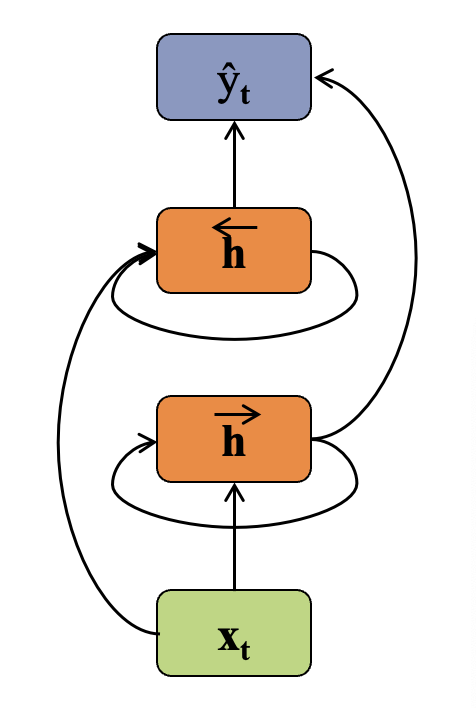
\includegraphics[width=5cm]{exam3/figures/brnn.png}}}
    \qquad
    \begin{aligned}
        \overrightarrow{\hv}_t &= \mathcal{H}(W_{x\overrightarrow{\hv}}\xv_t+W_{\overrightarrow{\hv}\overrightarrow{\hv}}\overrightarrow{\hv}_{t-1}+b_{\overrightarrow{\hv}}) \\ 
        \overleftarrow{\hv}_t &= \mathcal{H}(W_{x\overleftarrow{\hv}}\xv_t+W_{\overleftarrow{\hv}\overleftarrow{\hv}}\overleftarrow{\hv}_{t+1}+b_{\overleftarrow{\hv}}) \\ 
        \hat{y}_t &= W_{\overrightarrow{\hv}y}\overrightarrow{\hv}_t+W_{\overleftarrow{\hv}y}\overleftarrow{\hv}_t+b_y
    \end{aligned}
\end{align*}

\begin{subparts}
    \subpart[3] \textbf{Select all that apply:} Given sequences of length 3 of the form \\ $(\xv_1, y_1, \xv_2, y_2, \xv_3, y_3)$ which of the following quantities does $\overleftarrow{\hv}_2$ depend on?
    {%
    \checkboxchar{$\Box$} \checkedchar{$\blacksquare$} % change checkbox style locally
    \begin{checkboxes}
     \choice $\overrightarrow{\hv}_2$
     \choice $\xv_3$
     \choice $y_3$
     \choice $\hat{y}_3$
     \choice $\xv_1$
     \choice $W_{\overleftarrow{\hv}\overleftarrow{\hv}}$
     \choice None of the above
    \end{checkboxes}
    }
    \begin{soln}
        B, F
    \end{soln}

    \clearpage
    
    \subpart[3] \textbf{Select all that apply:} If the loss function is defined as \\ $\mathcal{L}=\sum_{t=1}^3 (y_t-\hat{y}_t)^2$, which of the following quantities does $\nicefrac{\partial \mathcal{L}}{\partial \overleftarrow{\hv}_2}$ depend on?
    {%
    \checkboxchar{$\Box$} \checkedchar{$\blacksquare$} % change checkbox style locally
    \begin{checkboxes}
     \choice $\nicefrac{\partial \mathcal{L}}{\partial \overleftarrow{\hv}_1}$
     \choice $\hat{y}_3$
     \choice $y_3$
     \choice $y_2$
     \choice $\nicefrac{\partial \mathcal{L}}{\partial W_{x\overrightarrow{\hv}}}$
     \choice $W_{\overleftarrow{\hv}y}$
     \choice None of the above
    \end{checkboxes}
    }
    \begin{soln}
        A, D, F
    \end{soln}
\end{subparts}
\begin{qauthor}
    Henry
\end{qauthor}
\end{parts}